\chapter{Introduction}

A large volume of data is generated daily on the Web in a variety of domains. These
data are often structured according to an organization's specific needs or formats: Leading to
a difficulty in integrating the data across the different applications.
These generated data might have to be associated with archival data, also of heterogeneous formats,
to provide a coherent view required by analysis tasks. Heterogeneous Web data formats, such as CSV or HTML, are not explicitly
defined to enable linking entities in one document to other related entities in external documents.

Based on W3C standard, semantic data formats such as RDF triples~\cite{intro_rdf}, are a solution to
this particular problem by enriching the data with knowledge and association across
different domains, through the use of common ontologies. RDF triples also form the basic building blocks of knowledge graphs.
Knowledge graphs are extensively used in social networks like Facebook\cite{facebook_linked_data}, IoT devices\cite{graph_of_things} and especially with Google's search
engine\cite{google_kg}, it enables machines to understand the data and perform complex automated processing
on the data. Considering the aforementioned scenarios, there is a need to transform these non-RDF data to RDF compliant formats on the fly while
new data are being generated. Furthermore, we would also like to apply stream operators on the input
before transforming, to enhance the enrichment of the data by applying operators on the incoming tuples.

There exists state-of-the-art techniques to solve the task of consolidating heterogeneous data
and transforming them to an RDF compliant format. In this thesis, we will focus on one such format called TURTLE.
These RDF transformation engines can be categorized into two major categories based on the type of input
which they consume; bounded and unbounded data input. Since we are focussing on the generation of RDF data
in a streaming environment, the class of RDF transformation engines on unbounded data will be of interest to our study.

Some engines support traditional stream operators like joins and aggregations. However, they do not consider
the characteristics of the streaming sources such as velocity and time-correlations between the different
input streams. This leads to a decline in the quality of the generated RDF triples. Moreover,
due to the nature of the infinite, continuous and real-time changing data of the streaming environment,
these operators have to be applied in the context of windows over a subset of the incoming data.
Clearly, with these restrictions and characteristics of the streaming sources, we need an adaptive approach
to applying these operators in windows.


\section{Terminologies}
This section will define and describe the different notations and terms used throughput
the rest of this work. We will elaborate more on RDF, RML and stream windowing for more
intuition behind the approach of this work.

\subsection{RDF}
Resource Definition Framework \cite{rdf_concepts} is a framework for representing data on the Web.
It portrays the data as a directed graph with the resources as nodes in the graph and the
edges as the relationship between the different resources.
Figure~\ref{fig:rdf_triple_ex} shows an example of an RDF triple statement describing
the information “John has an apple”.
The triple statement consists of the subject \textit{John}, the predicate \textit{has}
and the object \textit{apple}.

\begin{figure}[htbp]
    \centering
    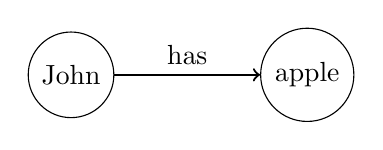
\begin{tikzpicture}[node distance={30mm}, main/.style = {draw, circle}]

        \node[main] (subject) {John};
        \node[main] (object) [right of=subject] {apple};

        \draw[->, thick] (subject) -- node[midway, above, sloped] {has} (object);

    \end{tikzpicture}
    \caption{An RDF triple representing the information “John has an apple”.}

    \label{fig:rdf_triple_ex}
\end{figure}


By composing these simple triple statements into a set of RDF triples, it yields us an RDF graph.
In Figure~\ref{fig:rdf_graph_ex}, 4 triple statements are composed together to form a
simple RDF graph describing \textit{John} and \textit{Mary} having the same \textit{apple}.
It might not be evident from the simple figures, about the advantages of
RDF graphs. Data representation in a graph model allows machines to follow the
\textit{links} between the resources, and discover more unknown
data in the linked knowledge graph. Link following is possible due to the nodes in
the triples being classified as one of the 3 different term types.

\begin{figure}[htbp]
\centering
\begin{tikzpicture}[node distance={30mm}, main/.style = {draw, circle}]

\node[main] (subject) {John};
\node[main] (subject_2) [below of=subject] {Mary};
\node[main] (object) [right of=subject] {apple};
\node[main] (apple_object_color) [above right of=object] {red};
\node[main] (apple_object_ripe) [below right of=object] {is ripe};
\node [cloud, draw,cloud puffs=10,cloud puff arc=120, aspect=2, inner ysep=1em]
(color_kg) [below right of=apple_object_color] {Colors KG};

\draw[->, thick] (subject) -- node[midway, above, sloped] {has} (object);
\draw[->, thick] (subject_2) -- node[midway, above, sloped] {has} (object);
\draw[->, thick] (apple_object_color) -- (color_kg);
\draw[->, thick] (object) -- node[midway, above, sloped] {has color} (apple_object_color);
\draw[->, thick] (object) -- node[midway, above, sloped] {ripeness} (apple_object_ripe);
\end{tikzpicture}
\caption{A simple RDF graph where the same “apple” is shared by both John and Mary.}
\label{fig:rdf_graph_ex}
\end{figure}

\subsubsection*{Term types}
Resources are classified into 3 different term types; IRI (Internationalized Resource Identifier),
literals and blank nodes. IRI can be regarded just like a web address


\subsection{RML}
RDF Mapping Language\cite{rml} is a superset of the W3C's R2RML which maps relational databases to
RDF datasets. RML improves upon R2RML by expressing mapping rules form heterogeneous
data sources and transforming them to RDF datasets whereas R2RML could only consume
data from relational databases.


